\documentclass{ivoa}
\input tthdefs

\usepackage{todonotes}
\usepackage{listings}
\lstloadlanguages{XML,sh,SQL}
\lstset{flexiblecolumns=true,tagstyle=\ttfamily, showstringspaces=False}

\ivoagroup{Edu IG}

\author{Molinaro, M.}
\author{Demleitner, M.}
\author{Ramella, M.}
\author{Iafrate, G.}

\editor{Molinaro, M.}

\SVN$Rev$
\SVN$Date$
\SVN$URL$

\previousversion{First published version}


\title{Educational Resources in the Virtual Observatory}

\begin{document}

\begin{abstract}

The goal of this IVOA Note is to introduce and explain practices followed
and requirements found while creating and 
deploying astrophysical resources 
dedicated to educational purposes ranging from pre-school outreach
material to courseware intended for active researchers
within the standard VO framework.
Issues, proposed solutions and desirables are here reported to be
possibly taken into account in future modifications of relevant
standards.



\end{abstract}


\section{Introduction}

Advances in technology and communications are creating new and exciting 
opportunities for teachers to bring astronomy into their 
classrooms.  As the VO makes science-grade data publicly available and
classroom sets of (suitably) networked PCs are now standard in schools,
exciting projects come within reach of teachers.  In order to make things 
happen, it is important to disseminate material to help teachers
tap into these resources.  These include documented step-by-step
tutorials, use cases explaining how to perform basic astrophysical research 
using VO tools and resources, and similar exist in various formats and
have been translated in different languages.

At the same time, the VO as used in research is a complex tool,
introducing many novel techniques.  To enable university level students
and active researchers to fully exploit the VO's capabilities, course
materials and worked-out use-cases have been found an efficient means of
developing the necessary skills far beyond interactive course situations
like ``VO Days''.  Efficient ways for interested users to locate such
material as well as for VO operators to curate it are highly desirable.

New opportunities also come on the observational side. 
There is a growing availability of remotely controlled 
telescopes dedicated to education in many countries world-wide, from the 
Bradford Robotic Telescope\footnote{\url{http://www.telescope.org}} on Mount
Teide, Tenerife 
to the radio telescopes of the Radio Physics
Lab\footnote{\url{http://www.ncra.tifr.res.in/rpl}}, IUCAA, Pune. 
In some cases, educational telescopes are 
linked into a network with the aim of guaranteeing the best observing conditions, 
including deep sky observations during regular daytime school hours, and 
the best instrument for the particular program of interest. Examples
of these networks are
iTelescope.net\footnote{\url{http://www.itelescope.net}} and
EuHOU-MW\footnote{\url{http://euhou.obspm.fr/public}}.



As telescopes enter classrooms more frequently, interest is growing for a 
public archive of observations and hence for publishing and curation tools, 
together with the basic applications needed to retrieve, display
and analyze data. The VO already includes most of the technology needed 
to satisfy the requests of educational observatories. In fact, since several 
years, VO, and in particular the European project EuroVO, is devoting part 
of its resources to
education\footnote{\url{http://wwwas.oats.inaf.it/aidawp5}}. It is 
therefore a natural decision for VO to tackle the problem of publishing 
educational data in VO archives.


Resource registration for both educational data services and documents 
is the most appropriate approach toward making educational resources 
available within the VO.  While
technically this may seem trivial, keeping too technical
research services out of the the resources devoted to education will
require some effort, that will also be needed in order to avoid contaminating 
VO professional research with obviously inadequate material.

In the next section we discuss the idea of educational resources curation, then 
we work out the use cases and needs for
registration of tutorials and documents. Finally, we discuss the idea of introducing language
internationalization in the resources.



\section{A Curated Registry for Education}

\label{sect:curreg}


From a technical point of view the registration of educational services
does not require extensions
to the existing for VOResource standard \citep{2008ivoa.spec.0222P}.
The only real need for investigating changes to what already exists is due to a
use case's distinction between resources to be used in teaching and dissemination
versus all the research driven resources that exist in the VO.



For simplicity here we will distinguish these two groups of resources as
\emph{educational}
 and 
\emph{professional}
 but without any intent of putting them
on different levels of importance.



\subsection{Educational vs. Professional Resources}

\label{sect:eduvspro}


On the one side, teachers and educators may find it difficult to filter out 
from all VO resources those that are suitable for their tutorials and
examples. On the other side, educational resources should not be retrieved 
by a standard professional query.
Given that it is not a matter of data quality, but only a distinction upon 
the resources' scope, nevertheless this duality leads to an issue about the
proper way to tag resources for educational usage.
  


In the next subsection we propose a possible tagging solution, based upon 
the existing 
\vorent{ContentLevel}
element of VOResource, but requiring a small change
to it. The subsequent subsection describes the idea of a
curated registry for educational resources and the reasons for it to exist.
  


\subsection{ContentLevel granularity issue}

\label{sect:contentlvl}

VOResource already has the 
\vorent{ContentLevel}
element
allowing data publishers to optionally identify their resources as being 
suitable for one or more of the following audiences:


\begin{itemize}

\item General{}

\item Elementary Education{}

\item Middle School Education{}

\item Secondary Education{}

\item Community College{}

\item University{}

\item Research{}

\item Amateur{}

\item Informal Education{}

\end{itemize}

This element turns out to be misused by many publishers, presumably because
it is not really clear what the subtle differences between the available
possibilities are; also, to require a fairly substantial enumeration to
convey ``for school use'' seems, in retrospect, not likely to promote
widespread adoption. We hence propose to simplify the content model
to:


\begin{itemize}

\item General{}

\item Research{}

\item Amateur{}

\end{itemize}

We expect this to reach two goals:
  
\begin{itemize}

\item to make publishers to better describe (on the average)
    their resources{}

\item to providing a tagging solution that suits a first filtering 
    on the resources at client level{}

\end{itemize}

Of course, the chance to 
add an 
\emph{Educational}
value option to this shrinked list, or even
substitute it to the 
\emph{General}
one, would be a valuable change.
  


This change in the already existing standard will require only 
a small effort to update already registered resources because nearly 97\% of 
them currently have \vorent{ContentLevel} set to 
\emph{research}, about 2\% of them have
no \vorent{ContentLevel} defined at all and only the remaining have a different value
(or set of values) set for this element (Appendix \ref{app:clcurrval} details better these
figures).
  

Until the change in VOResource can be performed, it
can work as a ``best practice'' recommendation, possibly even at a
registry level, where registries can map existing 
\vorent{ContentLevel} values 
  of 
\emph{University}
 to 
\emph{Research}
 and
  everything else except 
\emph{Amateur}
 to 
\emph{General}.
.


\subsection{Curating the Edu Registry}

\label{sect:edureg}


Even in the case of the simplified 
\vorent{ContentLevel}
tagging system
a curated registry for educational VO resources will be useful for
educators in order to let their students work with a registry without having to
worry about confusing material or overwhelming data sizes. A good example
for this is the educational version of the Aladin sky atlas that has a
built in, curated set of resources suitable for educational level 
tutorials.
  


Curation will require some effort in managing and keeping up to date
such a registry but, most important, it is subjected to  some restrictions coming from
the IVOA resource registry architecture. 
  


If such a registry were a standard publishing registry as laid down in
Registry Interfaces
\citep{2009ivoa.spec.1104B},
its resources would be harvested by the full registries: this means 
that any dedicated educational resource would end up in the full VO 
set of resources.  For reasons mentioned above, this is not
desirable.


If it were to be a full registry, it will harvest itself all the existing
resources, and not all of them will fit, or be suitable for, the educational
scope the registry has to be preserved for.
  


We need a resource (the curated, in Registry Interfaces
parlance, local, registry) capable of:
  
\begin{itemize}

\item 
\emph{selectively}
 harvesting the existing VO resources 
	(e.g., from a full registry);{}

\item register its own educational resources without being directly
	harvested by full registries (e.g., this could be done using a
	sibling publishing registry dedicated to host those educational
	resources that are to be harvested by the standard full registries.{}

\end{itemize}

This solution, also presented in Fig. 1, will not touch the existing architecture
while giving flexibility for the emerging educational resources to 
be curated.
  


\begin{figure}

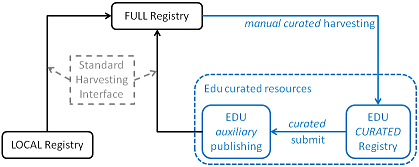
\includegraphics[width=0.9\textwidth]{curation.png}
\caption{Graphic illustration
    of the connecting interfaces between full registries and the educational
    curated one. The 
\emph{auxiliary}
 publishing is the only automatic token
    from the edu part.}
\label{fig:curation}
\end{figure}

\section{Registering Texts}

\label{sect:regext}

Educational material is not only about services – text-like material
like tutorials, worked-out use cases, or textbook-like material are at
least as important.  Within the VO community, there is a large body of
educational material for a wide variety of audiences ranging from pre-school to
researchers:

\begin{itemize}

\item EURO-VO AIDA WP5 - \url{http://wwwas.oats.inaf.it/aidawp5/eng_download.html}

\item EURO-VO Scientific Tutorials - \url{http://www.euro-vo.org/?q=science/scientific-tutorials}

\item VAO for Education - \url{http://virtualobservatory.org/education/}

\end{itemize}


To date, such material has been collected informally by the various
projects on plain web pages.  It is, in consequence, hard to find, with
knowledge of it often passed on antecdotically. In order to improve upon 
this situation, we
propose to keep record of educational material in the registry.

The VO already has a registry extension for standards, which of
course are also text-like, StandardsRegExt \citep{2012ivoa.spec.0508H}.  This extension,
however, focuses on metadata important for standards – e.g.,
vocabularies and status – that is not pertinent for educational
material.  Conversely, it is not concerned with document language (which
can safely be assumed to be English for standards), and it disregards
the issue of locating formatted and source versions, which for educational
material is important.  We therefore propose a simple registry extension
covering text-like material, dubbed DocRegExt.


\subsection{Use Cases}

\label{sect:regext-usecases}

The design of DocRegExt has been guided by the desire to fulfill the
following discovery cases:


\begin{itemize}

\item Is there a tutorial covering discovering intermediate mass black
holes? (Standard VOResource is sufficient){}

\item Is there a tutorial covering working with X-Ray data? (Standard
VOResource is sufficient){}

\item Is there a tutorial dealing with Planets suitable for school use?
(Standard VOResource is sufficient){}

\item Is there a tutorial dealing with Planets suitable for school use in
Italian? (That requires the declaration of the document language){}

\item What are the subjects of maintained (in the sense of: probably
working in the VO as found by the students) tutorials?
(The active flag of standard VOResource is
unsuitable here since even outdated resources will still be accessible;
therefore, we introduce the maintained flag){}

\item Are there tutorials using redshifts? (This is solved by allowing
table metadata in DocRegExt){}

\item Where can I find an editable version of tutorial ivo://auth/tut1?
(This is solved by allowing multiple access URLs with different content
types, which should be sufficient to allow answering the question){}

\item Are there translations of tutorial ivo://auth/tut2? (This is covered
by the recommendations on declaring relationships between text-like
resources){}

\item Is there material using service ivo://auth/svc1? (Again, declaring
relationships covers this use case){}

\item Is there material about something visible tonight? (In principle,
allowing the coverage element withing DocRegExt resources enables this
use case, although as of this writing, the Registry infrastructure does
not support spatial discovery).

\item I found this VO tutorial somewhere on the net (``on a mirror'').  Is it
the latest version?  If not, where can I find an update? (Unless the
title of the text changed, standard VOResource should suffice){}

\end{itemize}

An important additional use case is enabling an attractive, browsable
``roster'' of registred educational material.  A first attempt at such a
service is GAVO's VO Text Treasures (VOTT)
service\footnote{\url{http://dc.g-vo.org/VOTT}}.  It was found that one
requirement resulting from this use case is direct access to formatted
material in order to enable thumbnail generation.

On the use cases of locating editable forms of such texts – which
has been found to be necessary fairly regularly – we note in passing
that representing source-product relationships is in principle in the
domain of provenance and thus not in the Registry's main scope. However, in
the case discussed here the relation is so simple and its representation
so useful that we propose to include it in a DocRegExt.

\subsection{A Document Registry Extension}

\label{sect:regext-ext}

To satisfy the requirements derived above, we have designed a registry extension with
two definitions. First, we re-use the \vorent{vs:CatalogService} type
from VODataService 1.1 \citep{2010ivoa.spec.1202P} to construct
the \texttt{doc:Document} resource type.  

While the schema does not limit what kinds of capabilities a
\vorent{doc:Document} record has -- it is conceivable that tailored
services are communicated in this way --, access to actual files is
enabled using \vorent{doc:Edition}-typed capabilities.  It may be
argued that this use of VOResource capabilities stretches their
semantics a bit.  We argue, however, that these documents can well be
understood as parameterless service endpoints.  Using capabilities
furthermore allows a complete representation of the metadata in RegTAP
without any extra tables (cf.~sect.~\ref{sect:docregext-regtap}).

For reference, Appendix \ref{app:schema} contains a rendering of the
extension schema as of the publication of the note.  

The resource-level reference URL in \vorent{doc:Document} records should
be some sort of landing page with an abstract of the text and links to
the full texts and perhaps the document source(s).  When using the
versioned repository (sect.~\ref{sect:svn-repo}), this could be the
top-level README file within the VCS.  For simple documents, it is
acceptable to use the English-language document itself as
\vorent{referenceURL}; documents only available in non-English should
provide a landing page with an English-language abstract, though.

The \vorent{facility} and \vorent{instrument} items should only be set
if the text in question actually exploits particular properties of the
concrete instrument.  A \vorent{tableset} can be given for the central
table-like structures a text deals with and facilitates discovery by
physics via the UCDs given in the tableset.

Document-typed resource records should define relations to other
general resources (e.g., applications, services,\dots) 
they use.  VOResource 1.1 provides a vocabulary of possible
relationships. Document records should preferably use \emph{Cites} and
in particular declare relationships to tools.  If these are not
registred, use the name of their binary name as the name of the related
resource; this will very typically be lowercase-only.

Each \vorent{Edition}-typed capability should 
correspond to a translation of the document.  It
is recommended to list the English-language version first if it exists.

The following description of the \vorent{doc:Edition} capability
is generated from the schema file.

% GENERATED: !schemadoc DocRegExt-1.xsd Edition
\begin{generated}
\begingroup
      	\renewcommand*\descriptionlabel[1]{%
      	\hbox to 5.5em{\emph{#1}\hfil}}\vspace{2ex}\noindent\textbf{\xmlel{doc:Edition} Type Schema Documentation}

\noindent{\small
        An "edition" (typically: translation) of the document.
      \par}

\noindent{\small
        Although for a while, multiple editions of the document in one language
        may be given (corresponding perhaps to two "major versions), in
        general, only the latest version of the document per language should be
        given.

        At least one vr:WebBrowser-typed interface with 
        role="rendered" must be present. The access URL of the interface
        points to a rendered version of the edition (preferably in PDF, 
        but HTML is acceptable, too).

        Editors are strongly encourated to also provide an 
        interface with role="source", the accessURL of which should point
        to an editable version of the document, a version controlled
        repository, or the like.
      \par}

\vspace{1ex}\noindent\textbf{\xmlel{doc:Edition} Type Schema Definition}

\begin{lstlisting}[language=XML,basicstyle=\footnotesize]
<xs:complexType name="Edition" >
  <xs:complexContent >
    <xs:extension base="vr:Capability" >
      <xs:sequence >
        <xs:element name="language" type="xs:token" minOccurs="1"
                  maxOccurs="1" />
        <xs:element name="locTitle" type="xs:token" minOccurs="0"
                  maxOccurs="1" />
      </xs:sequence>
    </xs:extension>
  </xs:complexContent>
</xs:complexType>
\end{lstlisting}

\vspace{0.5ex}\noindent\textbf{\xmlel{doc:Edition} Extension Metadata Elements}

\begingroup\small\begin{bigdescription}\item[Element \xmlel{language}]
\begin{description}
\item[Type] string: \xmlel{xs:token}
\item[Meaning] 
                The language this document is (mainly) written in,
                as an RFC 3066 language code.
              
\item[Occurrence] required
\item[Comment] 
                The country codes must be given in all lowercase.  This
                results in strings like en-us, de-de, or es-mx.

                This language is also the language for locTitle, 
                irrespective or that element's xml:lang setting.
              

\end{description}
\item[Element \xmlel{locTitle}]
\begin{description}
\item[Type] string: \xmlel{xs:token}
\item[Meaning] 
\item[Occurrence] optional

\end{description}


\end{bigdescription}\endgroup

\endgroup
\end{generated}

% /GENERATED

\subsection{DocRegExt in RegTAP}
\label{sect:docregext-regtap}

In the relational registry \citep{2014ivoa.spec.1208D}, DocRegExt is
straightforwardly represented in the standard VOResource tables.  in
particular, to find all titles and access urls for documents, one would
write:

\begin{lstlisting}[language=SQL]
SELECT res_title, access_url FROM
  rr.resource 
  NATURAL JOIN rr.interface
WHERE
  res_type='doc:document'
  and intf_role='rendered'
\end{lstlisting}

The \vorent{language} and \vorent{locTitle} elements from the
\vorent{doc:Edition} capability extension are mapped into
\verb|res_details| with the following \verb|detail_xpath|s:

\begin{itemize}

\item \texttt{/capability/language} -- the document language as an RFC
3066 language code.
\item \texttt{/capability/locTitle} -- the title in the national
languate.
\end{itemize}

The downside of not defining an extra table for the documents is that
the query patterns in RegTAP are somewhat clumsy.  For instance, to list
the English and Italian titles of all texts available in Italian, one
has to carefully join two subqueries to \verb|res_details|:

\begin{lstlisting}[language=SQL]
SELECT res_title, loctitle FROM
  rr.resource 
  NATURAL JOIN (
    SELECT ivoid, loctitle FROM (
        SELECT ivoid, cap_index, detail_value as loctitle
        FROM rr.res_detail
        WHERE detail_xpath='/capability/locTitle') AS titles
      NATURAL JOIN (
        SELECT ivoid, cap_index 
        FROM rr.res_detail
        WHERE 
          detail_xpath='/capability/language'
          AND detail_value LIKE 'it_%') AS italiancaps
    ) as loctitles
WHERE
  res_type='doc:document'
\end{lstlisting}


Here is a (slightly abridged) example record (TBD: update this):

\lstinputlisting[language=XML,basicstyle=\footnotesize]{m1distance-example.xml}

\subsection{A versioned repository for tutorials}

\label{sect:svn-repo}

Registering text document as VO resources allows searching for tutorials
and similar 
material through standard registry interfaces, but keeping 
tutorials up to date, in their master form and also in their translated 
versions, is another important issue to allow proficient use.
A versioned repository (using subversion as the version control system) 
has been set up at GAVO data
center\footnote{\url{http://svn.ari.uni-heidelberg.de/svn/edu/}} 
and collects part of the
already existing VO tutorials with the goal of preserve them and let users 
update and translate them.
The repository has an internal structure that takes care for:

\begin{itemize}

\item different national languages (master language set to english){}

\item translation vs. master language updates{}

\item licensing, in order to clarify how and whether a tutorial can be changed or re-used{}

\item additional materials used by tutorials{}

\item access roles to allow everyone to access tutorials but prevent untrusted updates or additions to it{}

\end{itemize}

Details of this structure are discussed in a \texttt{README} file at the
root of the
repository\footnote{\url{http://svn.ari.uni-heidelberg.de/svn/edu/README}}.
The repository is intended to work as a space for cooperative 
VO tutorials development.




\appendix

\section{ContentLevel values summary}

\label{app:clcurrval}


This appendix reports some statistics on the usage of the ContentLevel 
element in \citep{2008ivoa.spec.0222P} as of 2014-01-30, taken from the
GAVO RegTAP endpoint http://dc.g-vo.org/tap .
There are 14392 useful resources (excluding authorities, standards and
similar) that expose 26 different values as their ContentLevel.
In table \ref{tab:cldist} these values are reported in order of count.



\begin{table}
\begin{tabular}{lp{12cm}}
\sptablerule
\textbf{count}&
\textbf{content\_level string}\\
\sptablerule
13937&research\\
290&\\
41&university research\\
40&general university research amateur\\
24&university\\
14&university research amateur\\
7&general\\
5&research general\\
4&general research\\
3&secondary education community college university research amateur\\
3&research university community college\\
3&elementary education middle school education secondary education\\
3&general university research\\
2&research university\\
2&research amateur university community college\\
2&general informal education\\
2&general elementary education middle school education secondary education community college university research amateur informal education\\
1&university community college research\\
1&general university research amateur informal education\\
1&elementary education middle school education secondary education community college university research\\
1&general secondary education university research\\
1&university research general informal education\\
1&research university amateur\\
1&elementary education middle school education secondary education community college university research amateur\\
1&elementary education middle school education secondary education community college university research amateur informal education\\
1&university research amateur informal education\\
1&general university research informal education\\
\end{tabular}
\caption{Empirical distribution of \vorent{ContentLevel}s declared by VO
resources.}
\label{tab:cldist}
\end{table}



This table can be easily updated from the same endpoint (or an analogue 
one) using the following ADQL query:

\begin{verbatim}
SELECT 
  count(*) as cnt, content_level
FROM 
  rr.resource
WHERE
  res_type not in ('vstd:servicestandard', 'vg:authority', 
    'vstd:standard', 'va:application', 'vr:organization')
GROUP BY content_level
ORDER BY cnt DESC
\end{verbatim}

The table shows that only about 1\% of the ContentLevel values use 
something different and more complex than 
\emph{research}, when 
the element is not empty. Morever, of this 1\% (165 resources), 
61 include the \emph{general} value (roughly 37\% of them), 
29 (17\%) state that are devoted to some 
\emph{education} level only,
while 148 (90\%) state that are also devoted to some 
\emph{education} level (up to 
\emph{university}).


\section{The proposed DocRegExt Schema}

\label{app:schema}

The following XML schema is given here for reference and convenience.
It should not be used in software development.  As long as the schema is
not formally endorsed by the IVOA, the authoritative version is the one
on
Volute\footnote{\url{https://volute.g-vo.org/svn/trunk/projects/edu/edumatters/DocRegExt-1.xsd}}.
We intend to have it endorsed by the IVOA, after which the canonical
source will be the IVOA schema repository.

\lstinputlisting[language=XML]{DocRegExt-1.xsd}

\bibliography{ivoatex/ivoabib,ivoatex/docrepo}

\end{document}
